\documentclass[12pt,a4paper]{article}

\usepackage{amsmath,amssymb,amsthm}
\usepackage{mathtools}
\usepackage{geometry}
\usepackage{hyperref}
\usepackage{microtype}
\usepackage{setspace}
\usepackage{enumitem}
\usepackage{tikz}
\usepackage{tikz-cd}
\usetikzlibrary{positioning,arrows,arrows.meta,calc,matrix}
\usepackage{booktabs}
\usepackage{array}
\usepackage{caption}
\usepackage{subcaption}
\usepackage{xcolor}
\usepackage{fontenc}
\usepackage{inputenc}

\geometry{
  top=1.1in,
  bottom=1.1in,
  left=1.25in,
  right=1.25in
}

\onehalfspacing

\hypersetup{
  colorlinks=true,
  linkcolor=black,
  citecolor=black,
  urlcolor=black
}

\theoremstyle{plain}
\newtheorem{theorem}{Theorem}[section]
\newtheorem{proposition}[theorem]{Proposition}
\newtheorem{lemma}[theorem]{Lemma}
\newtheorem{corollary}[theorem]{Corollary}

\theoremstyle{definition}
\newtheorem{definition}[theorem]{Definition}
\newtheorem{example}[theorem]{Example}
\newtheorem{remark}[theorem]{Remark}

\newcommand{\E}{\mathcal{E}}
\newcommand{\B}{\mathcal{B}}
\newcommand{\C}{\mathcal{C}}
\newcommand{\D}{\mathcal{D}}
\newcommand{\Hom}{\mathrm{Hom}}
\newcommand{\id}{\mathrm{id}}
\newcommand{\op}{\mathrm{op}}
\newcommand{\Type}{\mathrm{Type}}
\newcommand{\sign}{\mathrm{sign}}

\title{\textbf{The Geometry of Constraints}\\[0.6em]
\large Adversarial Representations, Fibrational Semantics,\\
and the Dependency Architecture of Formal Systems}

\author{Flyxion}

\date{}

\begin{document}

\maketitle
\thispagestyle{empty}

\begin{abstract}
This essay traces a structural continuity running from the empirical phenomenon of adversarial vulnerability in machine learning through the differential geometry of neural representation spaces, and ultimately to the categorical foundations of dependent type theory. Beginning with the observation that adversarial perturbations are not isolated anomalies but geometric features of learned representation manifolds, the essay develops a unified conceptual framework in which adversarial subspaces, Grothendieck fibrations, comprehension categories, and the $\lambda$-cube all emerge as manifestations of the same underlying architecture: a geometry of constraints governing how structures vary across contexts and interact across levels of abstraction. The Cox--Bunzel representational similarity framework and Centered Kernel Alignment are interpreted geometrically as instruments for probing the foliation structure of high-dimensional semantic manifolds. The $\lambda$-cube is reinterpreted not as a syntactic taxonomy but as the minimal coordinate system for a stratified dependency lattice, one whose axes correspond to adjunctions between levels of a formal hierarchy. Comprehension categories are shown to generate the cube's structure automatically from the minimal data of a fibration equipped with context extension. The essay concludes by proposing that type theory, categorical semantics, information geometry, and adversarial machine learning are all partial descriptions of a single geometry: the geometry of constraint fields defined over spaces of contexts.
\end{abstract}

\newpage
\tableofcontents
\newpage

%% ======================================================================
\section{Robustness, Regulation, and the Limits of Verification}
%% ======================================================================

Modern neural networks achieve predictive performance that would have appeared extraordinary a generation ago, yet they remain fragile in a manner that has no analogue in classical engineering systems. Minor manipulations of input data---manipulations that appear insignificant or even imperceptible to human observers---can produce large, discontinuous changes in model behavior. These adversarial perturbations are not isolated pathological cases. They occupy large, geometrically structured regions of the input space, and their existence is not contingent on implementation details of any particular architecture. They are, as the subsequent analysis will argue, necessary consequences of the geometry of learned representations in high-dimensional spaces.

This fragility has become a matter not merely of theoretical interest but of regulatory consequence. As artificial intelligence systems become embedded in critical infrastructure, financial decision-making, healthcare, and public governance, their resistance to adversarial manipulation becomes a precondition of responsible deployment. The European Union's AI Act requires organizations to demonstrate robustness and security as core properties of high-risk systems. Similar frameworks are emerging across multiple jurisdictions. Yet these regulatory demands run immediately into a mathematical obstacle: the adversarial attack surface of a deep neural network is combinatorially enormous, and complete verification of robustness with respect to that surface is computationally infeasible. Even verifying robustness within a small perturbation radius around a single input is NP-hard in the general case.

The central tension of adversarial machine learning research is therefore not primarily a tension between safe and unsafe systems but a tension between the theoretical completeness required by rigorous guarantees and the statistical coverage achievable in practice. Organizations cannot enumerate all adversarial inputs. They can only probe the adversarial landscape using surrogate methods and hope that their probes provide representative coverage. Understanding what ``representative'' means in this context requires understanding the geometry of representation spaces, which in turn opens onto mathematical structures far deeper than the applied setting might initially suggest.

This essay traces that depth. It begins with the applied problem of adversarial transferability and the representational similarity metrics developed to address it, then passes through the differential geometry of transformer attention mechanisms and high-dimensional embedding spaces, and ultimately arrives at Grothendieck fibrations, comprehension categories, and the $\lambda$-cube. The claim developed throughout is that these apparently disparate topics are unified by a single structural insight: complex systems, from neural networks to logical languages, can be understood as layered spaces of states, constraints, and meta-constraints, and the behavior of adversarial perturbations, program evaluation, and logical proof are all instances of motion through such layered spaces.

%% ======================================================================
\section{Adversarial Transferability and Representational Similarity}
%% ======================================================================

The phenomenon of adversarial transferability was among the first indications that adversarial vulnerability is a structural property of learned representations rather than an idiosyncratic flaw of individual architectures. Early work by Goodfellow, Shlens, and Szegedy established that neural networks exhibit large connected regions of input space in which small perturbations produce dramatic changes in output classification. These adversarial examples arise because the learned decision boundary of a network is highly nonlinear yet locally almost linear in high-dimensional regions. A perturbation aligned with the gradient of the loss function can push an input across the boundary with minimal displacement in input space. The fast gradient sign method formalizes this intuition: given a model $M$ with loss $L_M$ evaluated at input $x$, the perturbation
\[
\delta_M \;=\; \epsilon\,\sign\!\bigl(\nabla_x L_M(x)\bigr)
\]
produces an adversarial example $x + \delta_M$ that is geometrically close to $x$ yet behaviorally distant.

The transferability observation sharpened this understanding considerably. Adversarial examples crafted on one model frequently deceive other models trained on the same task, even when the architectures differ substantially. This cross-model transfer implies that adversarial directions are not idiosyncratic to individual networks but are aligned with structural features of the shared task geometry. An attack transfers from surrogate $S$ to target $T$ when the gradients are sufficiently aligned:
\[
\bigl\langle \nabla_x L_S(x),\; \nabla_x L_T(x) \bigr\rangle \;>\; 0.
\]
The question of when this alignment holds, and how to measure it without direct access to the target model, is the practical problem that representational similarity metrics are designed to address.

Centered Kernel Alignment (CKA) offers one principled answer. Given two networks $f$ and $g$ that map a common set of inputs to activation matrices $X$ and $Y$, CKA measures the similarity between the pairwise relationship structures induced by these activations. Formally, with $K = XX^\top$ and $L = YY^\top$,
\[
\mathrm{CKA}(K, L) \;=\; \frac{\|L^\top K\|_F^2}{\|K^\top K\|_F \,\|L^\top L\|_F},
\]
where centering is applied to remove mean effects. CKA produces a value in $[0,1]$ that is invariant to orthogonal transformations and isotropic scaling. High CKA similarity indicates that two networks organize data into similar geometric patterns within their representation spaces: they partition the input manifold into analogous clusters and impose analogous metrical relationships. Because adversarial vulnerabilities are closely tied to the geometry of learned representations, models with similar CKA scores are more likely to share adversarial directions.

The Cox--Bunzel framework operationalizes this observation into a testing protocol for organizations required to demonstrate adversarial robustness. The protocol partitions surrogate models into two groups based on their CKA similarity to the target model. The high-similarity group, characterized by CKA scores above approximately $0.55$ for convolutional architectures, provides proxy models that are geometrically close to the target; attacks generated on these surrogates are likely to transfer. The low-similarity group, with CKA scores below approximately $0.35$, ensures that the testing protocol also explores adversarial regions orthogonal to those shared with the high-similarity cluster. By combining attacks from both groups, the protocol approximates coverage of the adversarial landscape without attempting an impossible exhaustive search. The Diagonal Box Similarity metric supplements this global picture with layer-by-layer granularity, allowing comparison of local representation structure at different network depths.

This framework converts the theoretical impossibility of complete robustness verification into a tractable statistical testing problem. But to understand why this conversion works---why representational similarity should predict attack transferability---requires understanding the geometry of the representation spaces themselves.

%% ======================================================================
\section{The Geometry of Representation Spaces}
%% ======================================================================

Neural networks of sufficient capacity learn to map inputs into high-dimensional embedding spaces in which semantic relationships become approximately linear. The famous observation that word embedding spaces support vector arithmetic---that the displacement from ``king'' to ``queen'' resembles the displacement from ``man'' to ``woman''---reflects a deeper structural property: gradient-based training on semantic tasks tends to induce embedding geometries in which meaningful distinctions correspond to approximately linear directions. This approximate linearity is not incidental. It follows from the interaction between the loss landscape, the implicit biases of gradient descent, and the functional form of the network.

The resulting representation spaces are not smooth Riemannian manifolds in any classical sense. A neural network computes a piecewise smooth map from input space to representation space, assembled from compositions of affine maps and nonlinearities. The geometry of this map determines the network's sensitivity to perturbations. At a point $x$ in input space, the Jacobian
\[
J_M(x) \;=\; \frac{\partial h_M(x)}{\partial x}
\]
describes how small displacements in input space propagate into representation space. When $J_M(x)$ has large singular values along certain directions, small movements in those directions produce large changes in the representation, and consequently in the model's output. These high-gain directions constitute the adversarial subspace local to $x$.

Transformer architectures complicate this geometry in ways that are quantitatively significant. Attention mechanisms dynamically reweight contextual relationships between token representations, computing similarity relationships through scaled dot-product operations and normalizing through softmax. This process effectively induces a context-dependent metric over the representation manifold. Different inputs yield different attention patterns, and hence different effective metrics. The result is a representation space whose curvature varies dramatically across contexts.

The softmax aggregation inherent in attention also produces a distinctive geometric phenomenon: many distinct inputs can collapse onto nearly identical internal representations. Attention mechanisms aggregate value vectors through softmax-weighted combinations, which means that inputs producing similar query-key similarity patterns will produce similar value aggregations, even when the inputs themselves differ substantially. The representation space therefore contains broad regions of approximate equivalence---submanifolds along which the network's internal state remains nearly constant despite large variation in the input. The network has, in effect, learned to ignore certain directions of input variation.

These regions of approximate equivalence form structures resembling degenerate foliations. A foliation of a manifold is a decomposition into layered submanifolds of lower dimension, called leaves, that fit together without crossing. In a standard foliation the leaves are smooth and uniform; in the degenerate foliations that appear in neural representation spaces, the dimensionality and smoothness of the leaves vary across the space. Along directions tangent to the leaves, model behavior remains approximately invariant. Along directions transverse to the leaves---directions crossing from one leaf to another---small displacements produce large changes in model output. The adversarial perturbation problem is precisely the problem of finding these transverse directions efficiently.

%% ======================================================================
\section{Adversarial Subspaces as Degenerate Foliations}
%% ======================================================================

The foliation picture allows a precise geometric account of why adversarial examples exist and why they are so abundant. In the representation manifold of a trained network, model outputs remain approximately constant along directions tangent to the leaves of equivalence. These are the directions that the training process has rendered semantically inert: rotations, lexical paraphrases, irrelevant stylistic variations, pixel-level perturbations that do not affect the dominant features. Directions transverse to the leaves, however, are precisely those along which the network's output is sensitive. Because the ambient space is high-dimensional---modern transformer models operate in spaces of thousands to hundreds of thousands of dimensions---there exist vastly many directions transverse to any given leaf.

The adversarial subspace at a point $x$ can therefore be characterized as the set of directions in a neighborhood of $x$ that are approximately transverse to the local leaf through $x$. Because the leaf structure is degenerate---varying in dimension and regularity across the space---the adversarial subspace is not a smooth manifold but a stratified region with irregular boundaries. This accounts for the empirical observation that adversarial perturbations can be found efficiently in many directions from almost any input: the transverse cone is wide.

Transferability now has a geometric explanation. Two models share adversarial directions when their foliations have similar leaf structures in overlapping regions of input space. CKA similarity is a proxy for this geometric alignment: it measures whether two networks impose similar pairwise distances on the same inputs, which is equivalent to asking whether their local equivalence classes are organized similarly. High CKA implies that the two foliation structures are approximately aligned, so the transverse directions for one model are approximately transverse for the other. Low CKA implies that the foliations have drifted apart, so their respective transverse cones may be nearly orthogonal.

The scaling behavior of adversarial transferability follows naturally from this picture. As model size increases, several geometric changes occur in representation space. Larger models distribute semantic information across higher-rank feature manifolds: the Jacobian $J_M(x)$ develops a broader singular value spectrum, making the model sensitive along more directions. Simultaneously, independently trained large models tend to develop foliations whose orientations are less correlated. In high-dimensional spaces, the expected cosine similarity between two random vectors approaches zero:
\[
\mathbb{E}\!\left[\frac{\langle g_S,\, g_T\rangle}{\|g_S\|\,\|g_T\|}\right] \;\approx\; 0.
\]
When gradient directions behave like approximately random vectors in the high-dimensional tangent space, adversarial directions for different models become nearly orthogonal. Each large model possesses many vulnerable directions---because its high-dimensional representation space contains many sensitive directions---yet those directions are less aligned across models, so attacks transfer less effectively. The adversarial cones widen but rotate independently.

The ensemble defense strategy exploits this geometry directly. If the adversarial directions for each component model are approximately orthogonal, the intersection of all their adversarial subspaces is small. An attacker must find perturbations lying simultaneously in several differently oriented vulnerability cones, which is exponentially harder than attacking any single model. The deeper insight is that adversarial vulnerability is not primarily about the existence of sensitive directions---those are nearly inevitable in high-dimensional nonlinear systems---but about the correlation structure of those directions across models. Diversity in representation geometry, measured by CKA dissimilarity, translates directly into ensemble robustness.

%% ======================================================================
\section{The $\lambda$-Cube as a Coordinate System for Constraint Spaces}
%% ======================================================================

The geometric language developed to describe neural representation spaces---manifolds, foliations, sections, bundles---is not merely metaphorical. The same mathematical structures arise in the categorical semantics of dependent type theory, and understanding this connection reveals a deeper unity between adversarial machine learning, formal logic, and geometry.

The $\lambda$-cube is traditionally introduced as a diagram classifying typed $\lambda$-calculi by their expressive power. It is a cube whose vertices are type systems and whose edges represent the addition of a single expressive feature. From this perspective it appears to be primarily a taxonomy: a useful reference chart for the designers of programming languages and proof assistants. This presentation obscures what the cube actually represents.

At the deepest level, the $\lambda$-cube is a coordinate system for a space of dependency relations between levels of abstraction. Any typed formal system involves at least three levels: \emph{terms}, the executable expressions; \emph{types}, which classify terms; and \emph{kinds} (or universes), which classify types. The cube arises from asking a precise question about how these levels may depend on one another. Each of the three axes corresponds to one permitted cross-level dependency:

\begin{itemize}[leftmargin=2em]
\item \emph{Types depending on terms.} This axis introduces dependent types. When a type $B(x)$ may mention a specific term $x : A$, the type acts not as a static predicate but as a constraint whose shape varies with the position in the base space. The typing judgment $x : A \vdash B(x) : *$ describes a family of types parameterized by elements of $A$.

\item \emph{Terms depending on types.} This axis introduces polymorphism. A term $\Lambda\alpha.\, t$ abstracts over a type variable, producing an expression that inhabits a type for every type substituted for $\alpha$. Polymorphic terms are uniform sections across the entire universe of types.

\item \emph{Types depending on types.} This axis introduces type operators, allowing types to be constructed by applying higher-order type-level functions. A type operator $F : * \to *$ transforms one type into another; its existence requires that types themselves be treatable as objects manipulable by the formal language.
\end{itemize}

When no cross-level dependency is permitted, the result is the simply typed $\lambda$-calculus $\lambda_\to$, in which types and terms form completely separate strata. Each additional axis adds a cross-level dependency: $\lambda P$ adds term-to-type dependency; $\lambda 2$ adds type-to-term dependency; $\lambda\underline\omega$ adds type-to-type dependency. The cube's eight vertices enumerate all combinations of these three binary choices. At the top vertex, where all three dependencies are simultaneously present, lies the Calculus of Constructions $\lambda C$, the foundation of modern proof assistants.

\begin{figure}[h]
\centering
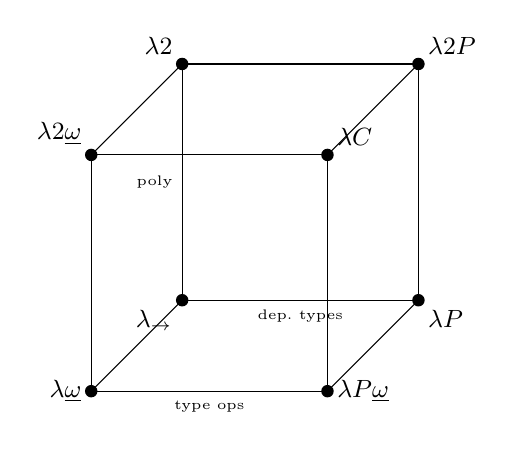
\begin{tikzpicture}[
  scale=1.5,
  node distance=2cm,
  every node/.style={font=\small},
  cube edge/.style={draw,thin}
]
  \coordinate (lto) at (0,0,0);
  \coordinate (lP)  at (2,0,0);
  \coordinate (l2)  at (0,2,0);
  \coordinate (lw)  at (0,0,2);
  \coordinate (lPw) at (2,0,2);
  \coordinate (l2P) at (2,2,0);
  \coordinate (l2w) at (0,2,2);
  \coordinate (lC)  at (2,2,2);

  \fill (lto) circle (1.5pt); \node[below left] at (lto) {$\lambda_\to$};
  \fill (lP)  circle (1.5pt); \node[below right] at (lP) {$\lambda P$};
  \fill (l2)  circle (1.5pt); \node[above left] at (l2) {$\lambda 2$};
  \fill (lw)  circle (1.5pt); \node[left] at (lw) {$\lambda\underline\omega$};
  \fill (lPw) circle (1.5pt); \node[right] at (lPw) {$\lambda P\underline\omega$};
  \fill (l2P) circle (1.5pt); \node[above right] at (l2P) {$\lambda 2P$};
  \fill (l2w) circle (1.5pt); \node[above left] at (l2w) {$\lambda 2\underline\omega$};
  \fill (lC)  circle (1.5pt); \node[above right] at (lC) {$\lambda C$};

  \draw[cube edge] (lto)--(lP) node[midway,below,font=\tiny]{dep.\ types};
  \draw[cube edge] (lto)--(l2) node[midway,left,font=\tiny]{poly};
  \draw[cube edge] (lto)--(lw);
  \draw[cube edge] (lP)--(l2P);
  \draw[cube edge] (lP)--(lPw);
  \draw[cube edge] (l2)--(l2P);
  \draw[cube edge] (l2)--(l2w);
  \draw[cube edge] (lw)--(lPw) node[midway,below,font=\tiny]{type ops};
  \draw[cube edge] (lw)--(l2w);
  \draw[cube edge] (lPw)--(lC);
  \draw[cube edge] (l2P)--(lC);
  \draw[cube edge] (l2w)--(lC);
\end{tikzpicture}
\caption{The $\lambda$-cube. Axes correspond to types depending on terms (depth), terms depending on types (height), and types depending on types (width). The Calculus of Constructions $\lambda C$ occupies the top vertex.}
\end{figure}

This interpretation of the cube as a coordinate system for dependency relations carries the key insight: the cube does not classify programming languages. It describes the minimal skeleton of cross-level dependency relations needed for a formal system to reason about objects, the constraints on those objects, and the constraints on those constraints. Any system capable of this threefold reflection must acquire structures equivalent to the three axes of the cube.

%% ======================================================================
\section{Comprehension Categories and the Emergence of the Cube}
%% ======================================================================

The fact that the $\lambda$-cube arises naturally from minimal categorical data---rather than being stipulated syntactically---is made precise by the theory of comprehension categories. A comprehension category provides the minimal structural account of the relationship between contexts, types, and terms, and from this account the cube's structure emerges automatically as the dependency skeleton of a self-describing formal system.

\begin{definition}[Comprehension Category]
A \emph{comprehension category} consists of a functor
\[
p \;:\; \E \;\longrightarrow\; \C^\to
\]
from a total category $\E$ to the arrow category of a base category $\C$, satisfying appropriate lifting and stability conditions. Equivalently, it consists of a fibration $p : \E \to \C$ together with, for every object $A$ lying over $\Gamma$ in $\E$, a chosen morphism
\[
\chi_A \;:\; \Gamma.A \;\longrightarrow\; \Gamma
\]
in $\C$, called the \emph{context extension} map, with the property that the pullback of $A$ along $\chi_A$ is the generic element of $A$.
\end{definition}

The base category $\C$ represents contexts: its objects are environments $\Gamma = (x_1 : A_1, \dots, x_n : A_n)$, and its morphisms are substitutions between contexts. The total category $\E$ contains dependent types together with their context information. The projection $p$ forgets the type and returns the context. A type judgment
\[
\Gamma \vdash A : *
\]
corresponds to an object $A \in \E$ with $p(A) = \Gamma$. The context extension $\Gamma.A$ is the context obtained by adding a fresh variable of type $A$; the comprehension map $\chi_A$ expresses the projection forgetting that variable.

This minimal structure already generates the fundamental operations of type theory through adjunctions. Given a substitution $f : \Delta \to \Gamma$ in the base, the fibration provides a reindexing functor
\[
f^* \;:\; \E_\Gamma \;\longrightarrow\; \E_\Delta
\]
that pulls types defined over $\Gamma$ back to types over $\Delta$. In syntactic terms, this is precisely substitution of terms for variables in a type expression.

Dependent products appear when this reindexing functor possesses a right adjoint:
\[
\Pi_f \;\dashv\; f^*.
\]
The right adjoint $\Pi_f$ maps a type $B$ over $\Delta$ to a type $\Pi_f B$ over $\Gamma$ that aggregates all coherent selections from $B$ over the preimage of each element of $\Gamma$. In logical terms this is universal quantification; in geometric terms it is the space of sections of a bundle. Dependent sums appear as the corresponding left adjoint:
\[
f^* \;\dashv\; \Sigma_f.
\]
The left adjoint $\Sigma_f$ constructs the total space of the bundle, pairing each base element with an element of its fiber. When both adjoints exist for every morphism in the base category, the comprehension category models a locally cartesian closed category---the categorical structure required for full dependent type theory.

Once this structure is in place, the three axes of the $\lambda$-cube emerge automatically from a single organizing question: how many levels of the comprehension structure are permitted to serve as bases for further comprehension? 

A system with only one level of objects---in which types cannot themselves be treated as terms---corresponds to the simply typed $\lambda$-calculus. Allowing types to serve as bases for further type families introduces the dependent type axis. Allowing types to parameterize terms polymorphically introduces the polymorphism axis. Allowing types to depend on other types introduces the type operator axis. The Calculus of Constructions arises when all three levels---terms, types, and the universe of types---may serve as base spaces for fibrations, and when the comprehension structure is closed under all three forms of dependency.

The cube is therefore not a classification imposed from outside but a structure that grows organically from the question of how many layers a comprehension category may contain and how those layers may depend on one another. In this sense it is not fundamentally about lambda calculus. It is the dependency skeleton of any self-describing formal system: any language capable of expressing objects, the constraints on those objects, and the constraints on those constraints must acquire structures equivalent to the three axes of the cube.

%% ======================================================================
\section{Grothendieck Fibrations and the Geometry of Dependent Types}
%% ======================================================================

The connection between type theory and Grothendieck fibrations is where the geometric interpretation of logic becomes fully explicit. A Grothendieck fibration formalizes the idea of objects varying over a base space in a way that captures the essential structure of substitution, context extension, and dependent quantification simultaneously.

\begin{definition}[Grothendieck Fibration]
A functor $p : \E \to \B$ is a \emph{Grothendieck fibration} if for every object $e \in \E$ and every morphism $f : b \to p(e)$ in $\B$, there exists a \emph{cartesian lifting}: a morphism $\bar f : \bar b \to e$ in $\E$ with $p(\bar f) = f$, through which every other morphism over $f$ factors uniquely.
\end{definition}

The base category $\B$ represents contexts or environments. The total category $\E$ contains objects that live over those contexts. For each base object $\Gamma$, the \emph{fiber category} $\E_\Gamma$ consists of all objects $e$ with $p(e) = \Gamma$ together with the vertical morphisms between them. The fiber over $\Gamma$ is the category of types in context $\Gamma$.

The correspondence with type-theoretic judgments is nearly perfect:
\begin{align*}
\Gamma \in \B \quad &\longleftrightarrow \quad \text{a context} \\
A \in \E_\Gamma \quad &\longleftrightarrow \quad \Gamma \vdash A : * \\
t \in \E_\Gamma(A, B) \quad &\longleftrightarrow \quad \Gamma \vdash t : A \to B
\end{align*}
A morphism $f : \Delta \to \Gamma$ in the base induces a reindexing functor $f^* : \E_\Gamma \to \E_\Delta$ whose existence follows from the cartesian lifting property. This reindexing functor is precisely substitution: it takes a type $A$ defined in context $\Gamma$ and produces the type $f^* A$ in context $\Delta$ obtained by replacing the variables of $\Gamma$ with the terms specified by $f$.

Dependent types acquire a sharp geometric meaning in this framework. The family judgment $x : A \vdash B(x) : *$ describes an object $B$ in the total category lying over the projection
\[
p_A : \Gamma.A \to \Gamma.
\]
Geometrically, $B$ is a bundle over the base space $A$ whose fiber at each element $a : A$ is the type $B(a)$. A term $\Gamma \vdash t : \Pi_{x:A} B(x)$ is a section of this bundle: a coherent choice of one element from each fiber. The dependent product $\Pi_{x:A} B(x)$ is the object in $\E_\Gamma$ representing the space of all such sections, and it arises as the right adjoint of the reindexing functor along the projection $p_A$:
\[
\begin{tikzcd}
\E_{\Gamma.A} \arrow[r, shift left=2, "\Pi_{p_A}"] & \E_\Gamma \arrow[l, shift left=2, "p_A^*"'] \arrow[l, phantom, "\dashv"]
\end{tikzcd}
\]

The Grothendieck construction makes this structure visible at the level of the entire fibration. Given a functor $F : \B^\op \to \mathbf{Cat}$ assigning a category $F(\Gamma)$ of types to each context $\Gamma$, the Grothendieck construction produces the total category $\int F$ whose objects are pairs $(\Gamma, A)$ with $A \in F(\Gamma)$, and whose morphisms $(\Delta, B) \to (\Gamma, A)$ are pairs $(f, g)$ with $f : \Delta \to \Gamma$ and $g : B \to f^* A$. The projection $\int F \to \B$ forgetting the second component is automatically a Grothendieck fibration.

Sheaf semantics enrich this picture further. In sheaf theory, one studies objects that vary continuously over a topological space, assigning compatible objects to open regions such that assignments agree on overlaps and glue consistently to global sections. Type theory under the fibration interpretation behaves analogously. A context acts like an open region of a base space, a type describes how objects vary across that region, and a term inhabiting a type is a consistent section. Logical reasoning becomes the process of constructing global sections from local constraints: proofs demonstrate that locally defined type-theoretic data glue coherently across the entire base space.

Under this interpretation, programs become sections of fibrations over spaces of contexts, and evaluation corresponds to moving through the base space while maintaining compatibility between fibers. The subject-reduction property of typed calculi---which ensures that evaluation preserves typing---is precisely the condition that the evaluation flow remains within the fibers of the fibration: the trajectory stays on the constraint manifold.

%% ======================================================================
\section{The $\lambda$-Cube as a Lattice of Adjunctions}
%% ======================================================================

The deepest way to understand the $\lambda$-cube is through the lens of adjoint functors. When the cube is interpreted not as a diagram of syntactic systems but as a coordinate system for categorical structures, its axes correspond to distinct adjoint pairs becoming available inside the internal language.

The simplest case is the simply typed $\lambda$-calculus $\lambda_\to$. Its categorical semantics lives in a cartesian closed category. In this setting, the function type $A \to B$ corresponds to the exponential object $B^A$, and the currying isomorphism
\[
\Hom(X \times A,\, B) \;\cong\; \Hom(X,\, B^A)
\]
expresses the adjunction $(- \times A) \dashv (-)^A$. The $\lambda$-abstraction rule is the internal language of this adjunction: to give a function from $A$ to $B$ is the same as to give, in an extended context, an element of $B$.

Moving along the dependent-type axis introduces a family of adjunctions indexed by context projections. For each projection $p_A : \Gamma.A \to \Gamma$, the system must support both
\[
\Sigma_{p_A} \;\dashv\; p_A^* \;\dashv\; \Pi_{p_A},
\]
where $p_A^*$ is reindexing along the projection, $\Sigma_{p_A}$ is the left adjoint constructing total spaces, and $\Pi_{p_A}$ is the right adjoint constructing section spaces. The transition from cartesian closed categories to locally cartesian closed categories precisely corresponds to this axis: every slice category must support its own cartesian closed structure, allowing dependent products and sums to vary with the context.

Moving along the polymorphism axis introduces the ability to quantify over the universe of types. In categorical terms this requires the universe $U$ to be treated as an object in the category, and polymorphic terms to correspond to natural transformations---morphisms that are uniform across all instantiations of the type variable. This introduces a further adjunction between the functor of ``trivially indexed families'' and the functor extracting the underlying single type.

Moving along the type-operator axis allows types to be manipulated by higher-order type-level functions. Categorically, this requires the category to support internal hom-objects at the level of types, introducing exponentials between kinds and hence another adjoint structure at the meta-level.

The Calculus of Constructions $\lambda C$ occupies the vertex at which all three adjoint structures coexist simultaneously. At that point the internal language can form dependent products and sums, quantify over type variables polymorphically, and apply type-level functions, all within a single unified grammar. The Curry--Howard--Lambek correspondence makes the full triangulation explicit:
\begin{center}
\begin{tabular}{ccc}
\toprule
\textbf{Logic} & \textbf{Type Theory} & \textbf{Category Theory} \\
\midrule
Propositions & Types & Objects \\
Proofs & Terms & Morphisms \\
Universal quantification & $\Pi$-type & Right adjoint to reindexing \\
Existential quantification & $\Sigma$-type & Left adjoint to reindexing \\
Implication & Function type & Exponential / internal hom \\
Substitution & $\beta$-reduction & Adjoint transpose \\
\bottomrule
\end{tabular}
\end{center}

This adjoint lattice extends naturally beyond three dimensions. Each additional feature of modern type theory introduces a new adjoint pair. Modal type theories arise from adjunctions between modalities and inclusion functors. Linear type theories arise from adjunctions between the tensor product and the linear internal hom. Universe hierarchies $\Type_0 : \Type_1 : \Type_2 : \cdots$ arise from adjunctions between universe levels, replacing the single box-sort of the classical cube with an infinite tower of contexts. The $\lambda$-cube is therefore a three-dimensional section through a much larger structure: the full adjoint lattice governing all possible forms of typed computation. It is the most visible cross-section precisely because it is the minimal one that contains all three fundamental modes of dependency.

%% ======================================================================
\section{Type Theory as Information Geometry}
%% ======================================================================

Once the $\lambda$-cube is interpreted geometrically as a space of constraints and flows, it becomes natural to compare its structure with the manifolds studied in information geometry and statistical field theory. The comparison reveals that typed computation and statistical inference share a common geometric skeleton.

In information geometry, a statistical model is represented as a Riemannian manifold whose coordinates parameterize probability distributions. A point on the manifold corresponds to a particular distribution; a curve corresponds to a continuous transformation of that distribution. The Fisher information metric equips the manifold with an intrinsic notion of distance, and divergence measures such as the Kullback--Leibler divergence define the geodesic structure. Learning and inference are then described as motion through this manifold, guided by gradients of information measures.

The typing judgment
\[
\Gamma \;\vdash\; t : T
\]
can be interpreted in a parallel way. The context $\Gamma$ specifies a coordinate system, $T$ defines a constraint surface within the space of program states, and the judgment asserts that $t$ lies on that surface. The space of all program states forms an ambient configuration space, and types partition this space into constraint manifolds. Under this interpretation, a type is not merely a label but a geometric object: a submanifold of the state space defined by the type's constraints.

Beta reduction in the $\lambda$-calculus then resembles a dynamical flow on this space. Each reduction step transforms a term while preserving its type, because subject reduction guarantees type preservation throughout evaluation. The reduction flow is therefore constrained to remain on the constraint manifold defined by the type. The flow is not random but follows the rewriting rules of the calculus, which define a directed partial order on terms: the normal form, when it exists, is the stable equilibrium of the flow.

Dependent types introduce fiber bundle structure into this picture. A family of types $x : A \vdash B(x)$ defines a bundle over the base manifold $A$ whose fiber over each element $a$ is the constraint manifold $B(a)$. A dependent function of type $\Pi_{x:A} B(x)$ is a section of this bundle: it assigns to each point $a \in A$ an element of the fiber $B(a)$, consistently across the base. This is the exact structure of a physical field: a field of type $\Pi_{x : M} F(x)$ assigns to each spacetime event $x$ an element of the field fiber $F(x)$ above that event. Classical electromagnetism, for instance, assigns to each spacetime event a value of the electromagnetic field, which is an element of a fiber determined by the gauge structure of the theory. The parallel is not merely suggestive; the categorical structures are identical.

Under this field-theoretic interpretation, the $\lambda$-cube describes which kinds of fields over constraint manifolds are permitted:

\begin{itemize}[leftmargin=2em]
\item The dependent-type axis allows constraint manifolds (types) to depend on program states (terms). The shape of the fiber varies with the base point, producing a genuine bundle rather than a product.

\item The polymorphism axis allows computational trajectories (terms) to depend on the manifold itself (types). Polymorphic programs are sections that are uniform across the entire universe of constraint manifolds.

\item The type-operator axis allows manifolds to depend on other manifolds. Type constructors become operators transforming one constraint manifold into another, introducing a hierarchy of constraint spaces.
\end{itemize}

The Calculus of Constructions is the point where all three forms of field-theoretic dependency are simultaneously possible: it can express fields over fields over fields, allowing constraints, programs, and meta-structures to interact recursively. In information-geometric terms, the system can describe statistical models over statistical models over statistical models---manifolds parameterized by manifolds.

This interpretation resolves a puzzle about why type theory appears in such disparate domains. Proof assistants use it because it provides a language for expressing mathematical structures and their proofs within a single formal system. Cognitive scientists use it because it provides a language for describing hierarchically structured belief systems and their updates. Physicists use it because, in the form of homotopy type theory, it provides a synthetic language for homotopy theory and derived geometry. In all these cases the underlying reason is the same: any domain requiring formal description of structured transformations that preserve constraints across multiple levels of abstraction naturally acquires the geometry of the $\lambda$-cube.

%% ======================================================================
\section{Homotopy Type Theory and the Extension Beyond the Cube}
%% ======================================================================

Homotopy type theory (HoTT) demonstrates that the geometric interpretation of type theory is not merely metaphorical but can be pushed to the point where the logic of type theory and the logic of homotopy theory become provably equivalent. In HoTT, types are interpreted as topological spaces, elements as points, and equality proofs as paths. The identity type $\mathrm{Id}_A(a, b)$ is interpreted as the space of paths from $a$ to $b$ in $A$. Higher identity types---equalities between equalities---correspond to surfaces connecting paths, and so on through all dimensions.

Under this interpretation, dependent types become genuine fibrations in the topological sense. A family $x : A \vdash B(x)$ is interpreted as a continuous map from the total space $\sum_{x:A} B(x)$ to the base $A$, equipped with the standard lifting properties of a fibration. The fundamental group of the base space is reflected in the identity type: homotopy invariants of $A$ can be computed entirely within the type system.

The univalence axiom of HoTT asserts that equivalent types are identical. In categorical terms, this means that the identity type of the universe of types is homotopy equivalent to the space of type equivalences. This makes the universe behave like a classifying space: paths in the universe correspond to equivalences between types, surfaces correspond to natural isomorphisms, and higher-dimensional cells correspond to higher coherences. The universe therefore carries a rich geometric structure that the type system can describe and reason about internally.

The $\lambda$-cube is a shadow of this richer structure. It describes the dependency skeleton at a fixed level of homotopy---the level at which types are sets, where all identity proofs are trivially equal. HoTT relaxes this restriction, allowing types to have nontrivial homotopy groups, and thereby introduces an infinite tower of additional dependency relations: paths depending on points, surfaces depending on paths, and so on. Each dimension introduces a new fibrational structure beyond the three axes of the cube.

Higher topos theory provides the categorical framework for this extension. An $(\infty,1)$-topos is a category whose internal language is precisely HoTT: its objects are spaces (up to homotopy equivalence), its morphisms are continuous maps, and its internal logic is homotopy type theory. The $\lambda$-cube describes the internal language of an ordinary topos---the $0$-dimensional case---while HoTT describes the internal language of an $(\infty,1)$-topos, the fully homotopy-coherent case. Between these extremes lie the internal languages of $n$-toposes for each natural number $n$, forming an infinite hierarchy extending the cube in a direction orthogonal to all three of its original axes.

Derived algebraic geometry extends this picture further. In derived geometry, spaces carry additional structure from homological algebra: they are described not merely by their points and paths but by cochain complexes encoding their deformation theory. The types of derived geometry correspond to $\infty$-groupoids enriched in chain complexes, and the internal logic governing them requires yet additional fibrational structure beyond HoTT. The $\lambda$-cube therefore appears, in the longest view, as the minimal coordinate patch of an infinite-dimensional space of type theories parameterized by their homotopical dimension and homological depth.

%% ======================================================================
\section{Returning to Machine Learning: Representation Fields and Constraint Geometry}
%% ======================================================================

The foregoing analysis began with the empirical observation that adversarial vulnerability is a geometric property of learned representation spaces and then moved progressively toward the categorical and type-theoretic structures that formalize the geometry of constraint spaces. The final section returns to the starting point, now equipped with the abstract framework, to show how the two perspectives illuminate each other.

A trained neural network defines a representation field over its input space. At each input $x$, the network's internal state $h_M(x) \in \mathbb{R}^d$ can be thought of as a section value---the value that the network's representation field assigns to the point $x$ in input space. The training process shapes this field to assign similar values to semantically similar inputs, thereby encoding the task geometry in the structure of the field.

Under the fibration interpretation, the network's representation can be described as a section of a bundle over input space. The base space is the domain of possible inputs; the fibers are the high-dimensional representation spaces; and the network's learned weights determine a specific section---a continuous assignment of a representation to each input. The smoothness and structure of this section determine the network's behavior under perturbation.

Adversarial examples arise when this section has locally degenerate structure: when nearby inputs are assigned representations that are nearly identical in many directions but radically different in a few critical directions. In fibrational language, the section has near-zero variation along the leaves of the foliation but large variation in the transverse directions. This is the geometric condition for adversarial vulnerability: the section is locally ``flat'' in a degenerate sense, with large gradients concentrated in a few directions.

The CKA framework for measuring representational similarity is therefore a probe of fibrational alignment between two networks. High CKA similarity between models $f$ and $g$ indicates that their respective sections organize the input manifold into similar geometric patterns. The fibers assigned to any given input are related by approximately linear transformations that preserve pairwise inner products. This geometric alignment between sections predicts alignment of adversarial directions: if the sections vary steeply in similar directions, the adversarial transverse cones will be similarly oriented, and attacks will transfer.

The Cox--Bunzel testing protocol is, in this language, a strategy for obtaining representative coverage of the adversarial cone without exhaustively searching it. By sampling surrogates from both the high-CKA cluster and the low-CKA cluster, the protocol ensures coverage of directions both aligned with and orthogonal to the target's primary adversarial subspace. The statistical guarantee provided by this protocol is a statement about section overlap: it ensures that the evaluated attack directions span a geometrically diverse subset of the full adversarial cone.

The scaling behavior of adversarial transferability receives an information-geometric interpretation. Larger models define higher-rank sections: their Jacobians have broader singular value spectra, meaning the representation field varies steeply in more directions. But the direction of steepest variation is determined by the random initialization and training trajectory as much as by the architecture. As models scale, the alignment between their adversarial directions decreases---the sections become richer but their gradients become less correlated. In the field-theoretic picture, scaling produces a richer field with more independent degrees of freedom, and two rich fields are less likely to have aligned gradients than two impoverished ones.

This picture suggests a connection to the renormalization group in statistical physics, where the behavior of field theories at different scales is studied by integrating out short-distance degrees of freedom and observing how the resulting effective theory changes. In neural networks, the process of increasing model size and then applying regularization (through dropout, weight decay, or other means) could be interpreted as a field-theoretic renormalization: the effective representation field at the scale of the regularized model is a coarse-grained version of the full high-rank field. The adversarial transferability decrease at large scales may reflect the fact that large models possess non-renormalizable field-theoretic degrees of freedom---gradient directions that cannot be described by a simple low-dimensional effective theory shared across architectures.

%% ======================================================================
\section{Convergence: The Geometry of Constraints}
%% ======================================================================

The essay has traced a path from adversarial examples through representation geometry, foliation theory, categorical semantics, Grothendieck fibrations, comprehension categories, the $\lambda$-cube, information geometry, and homotopy type theory. The diversity of these topics conceals a structural unity that the foregoing analysis has progressively revealed.

The unity can be stated as a single organizing claim: complex systems---whether machine learning models, typed programming languages, or mathematical proof systems---are best understood as layered spaces of states, constraints, and meta-constraints, and the phenomena characteristic of each domain are instances of motion through such layered spaces under the governance of their constraint geometry.

In machine learning, states are input representations, constraints are the typing-like conditions imposed by training objectives and architectural inductive biases, and adversarial vulnerability is the existence of transverse directions along which small motion produces large change in behavioral category. Robustness evaluation is the problem of characterizing the geometry of these transverse directions without complete knowledge of the full constraint field.

In type theory, states are program terms, constraints are types (which are constraint manifolds in the state space), and computation is motion along those manifolds governed by reduction rules. The $\lambda$-cube describes the minimal configuration of cross-level dependencies needed for a language to reason about itself: to describe not only its states but also the constraints on those states and the constraints on those constraints.

In categorical semantics, the same structure appears as a Grothendieck fibration: a functor from a total category of constrained objects to a base category of contexts, equipped with reindexing functors and their adjoints. The fibration encodes, in categorical language, exactly the structure of substitution, dependent quantification, and context extension that type theory requires syntactically.

In information geometry, the structure appears as a family of statistical manifolds parameterized by a base space of models, with sections corresponding to consistent statistical inferences across the family. The connection to type theory is not merely analogy: both frameworks describe spaces of constraints organized over base spaces of contexts, and both treat the construction of global coherent objects from local constraints as the central operation.

The $\lambda$-cube functions as the simplest recognizable cross-section of this geometry. Its three axes are the three minimal cross-level dependencies needed for a formal system to be self-describing. The comprehension category generates the cube from even more minimal data, showing that the cube's structure is not stipulated but arises inevitably from the structure of a category of contexts equipped with a fibration and context extension. Grothendieck fibrations and sheaf semantics reveal the fully geometric content of this structure. Homotopy type theory extends it into an infinite-dimensional space of type theories parameterized by homotopical dimension.

The adversarial machine learning problem, which provided the essay's starting point, can now be situated within this framework as a special case of a general geometric problem: understanding how sections of high-dimensional constraint fields degenerate near their boundaries, where small transverse displacements produce large changes in behavioral category. The techniques developed for this problem---CKA-based representational similarity, surrogate partitioning, diagonal box metrics---are instruments for probing the geometry of learned constraint fields. The challenge of AI robustness is, at its deepest level, the challenge of understanding and controlling the geometry of representation spaces as constraint fields over the manifold of possible inputs.

What appears initially as a collection of unrelated technical tools---adversarial testing frameworks, dependent type systems, categorical fibrations, information geometry---is, under the analysis developed here, a collection of partial descriptions of the same underlying mathematical object: a geometry of constraints governing how structures vary across contexts and interact across levels of abstraction. The $\lambda$-cube, Grothendieck fibrations, and neural representation manifolds are, each in their own register, charts for different regions of this geometry. The enterprise of understanding any one of them in depth is, in the end, the same enterprise as understanding all the others.

%% ======================================================================
\begin{thebibliography}{99}

\bibitem{goodfellow2015} Goodfellow, I., Shlens, J., and Szegedy, C. (2015). Explaining and harnessing adversarial examples. \textit{International Conference on Learning Representations}.

\bibitem{szegedy2014} Szegedy, C., et al. (2014). Intriguing properties of neural networks. \textit{International Conference on Learning Representations}.

\bibitem{kornblith2019} Kornblith, S., Norouzi, M., Lee, H., and Hinton, G. (2019). Similarity of neural network representations revisited. \textit{Proceedings of the 36th International Conference on Machine Learning}, 3519--3529.

\bibitem{papernot2016} Papernot, N., McDaniel, P., and Goodfellow, I. (2016). Transferability in machine learning: From phenomena to black-box attacks using adversarial samples. \textit{arXiv preprint arXiv:1605.07277}.

\bibitem{coxbunzel} Cox, B. and Bunzel, A. (2024). Adversarial robustness evaluation and representational similarity. Manuscript.

\bibitem{euaiact} European Parliament and Council (2024). \textit{Regulation on Artificial Intelligence (AI Act)}. Official Journal of the European Union.

\bibitem{barendregt1992} Barendregt, H. (1992). Lambda calculi with types. In \textit{Handbook of Logic in Computer Science}, Vol.~2. Oxford University Press.

\bibitem{jacobs1999} Jacobs, B. (1999). \textit{Categorical Logic and Type Theory}. Elsevier.

\bibitem{grothendieck1960} Grothendieck, A. (1960). \'{E}l\'{e}ments de g\'{e}om\'{e}trie alg\'{e}brique. \textit{Publications Math\'{e}matiques de l'IH\'{E}S}, 4:5--214.

\bibitem{streicher1991} Streicher, T. (1991). \textit{Semantics of Type Theory}. Birkh\"auser.

\bibitem{hofmann1994} Hofmann, M. (1994). On the interpretation of type theory in locally cartesian closed categories. \textit{Computer Science Logic}, Lecture Notes in Computer Science.

\bibitem{univalent2013} Univalent Foundations Program (2013). \textit{Homotopy Type Theory: Univalent Foundations of Mathematics}. Institute for Advanced Study.

\bibitem{lurie2009} Lurie, J. (2009). \textit{Higher Topos Theory}. Princeton University Press.

\bibitem{amari2016} Amari, S. (2016). \textit{Information Geometry and Its Applications}. Springer.

\bibitem{atiyah1989} Atiyah, M. (1989). Topological quantum field theory. \textit{Publications Math\'{e}matiques de l'IH\'{E}S}, 68:175--186.

\bibitem{lawvere1969} Lawvere, F.W. (1969). Adjointness in foundations. \textit{Dialectica}, 23(3--4):281--296.

\bibitem{seely1984} Seely, R. (1984). Locally cartesian closed categories and type theory. \textit{Mathematical Proceedings of the Cambridge Philosophical Society}, 95:33--48.

\bibitem{coquand1988} Coquand, T. and Huet, G. (1988). The Calculus of Constructions. \textit{Information and Computation}, 76(2--3):95--120.

\bibitem{voevodsky2010} Voevodsky, V. (2010). Univalent foundations project. \textit{Unpublished manuscript}.

\bibitem{triantafillou2021} Triantafillou, E., et al. (2021). Representation similarity in neural networks: A review. \textit{Advances in Neural Information Processing Systems}.

\end{thebibliography}

\end{document}
